%%% Preamble
\documentclass[paper=a4,fontsize=11pt]{report}

\usepackage[utf8]{inputenc}
\usepackage[T1]{fontenc}
\usepackage{fourier}
\usepackage[french]{babel}
\usepackage[protrusion=true,expansion=true]{microtype}	
\usepackage{amsmath,amsfonts,amsthm} % Math packages
\usepackage[pdftex]{graphicx}	
\usepackage{url}
\usepackage{pdfpages}
\usepackage{todonotes}
\usepackage[a4paper, body={16cm,23cm},margin=1cm]{geometry}
\usepackage{float}
\usepackage{framed}
\usepackage[toc,page]{appendix} 
\usepackage{multicol}
\usepackage{colortbl}
\usepackage{pgfplotstable}

%%% Custom sectioning
\usepackage{sectsty}
\allsectionsfont{  \normalfont\scshape}
%\allsectionsfont{\centering \normalfont\scshape}

%%% Custom headers/footers (fancyhdr package)
\usepackage{fancyhdr}
\pagestyle{fancyplain}
\fancyhead{}								% No page header
\fancyfoot[L]{}							% Empty 
\fancyfoot[C]{}							% Empty
\fancyfoot[R]{\thepage}					% Pagenumbering
\renewcommand{\headrulewidth}{0pt}		% Remove header underlines
\renewcommand{\footrulewidth}{0pt}		% Remove footer underlines
\setlength{\headheight}{13.6pt}


%%% Equation and float numbering
\numberwithin{equation}{section}		% Equationnumbering: section.eq#
\numberwithin{figure}{section}		% Figurenumbering: section.fig#
\numberwithin{table}{section}		% Tablenumbering: section.tab#


%%% Define new commands
\newcommand{\horrule}[1]{\rule{\linewidth}{#1}} 	% Horizontal rule
\renewcommand{\bf}[1]{\textbf{#1}}
\renewcommand{\it}[1]{\textit{#1}}
\newcommand{\bfit}[1]{\textbf{\textit{#1}}}

\newcommand{\Todo}[1]{\todo[inline]{#1}}
\renewcommand{\thesection}{\thepart .\arabic{section}}

\usepackage{cases}
\usepackage{color}
\usepackage{xcolor}
\usepackage{relsize}

\usepackage{caption}
\DeclareCaptionFont{white}{\color{white}}
\DeclareCaptionFormat{listing}{\colorbox{gray}{\parbox{\textwidth}{#1#2#3}}}
\captionsetup[lstlisting]{format=listing,labelfont=white,textfont=white}

\usepackage[numbered]{mcode}

\lstset{breaklines=true,columns=fullflexible}
\colorlet{shadecolor}{black!10}

\delimitershortfall-1sp
\newcommand\abs[1]{\left|#1\right|}

%%% Begin document
\begin{document}

\includepdf[pages={1}]{title.pdf}

\tableofcontents

\listoftodos

\newpage

%%%%%%%%%%%%%%%%%%%%%%%%%%%%%%%%%%%%%%%%%%%%%%%%%%%%%%%%%%%%%%%%%%%%%%%%%%%%%%%%%%%%%%%%%%%%%%%%%%%%%%%%%%%%%%%%%%%%%%%%%%%
%%%%%%%%%%%%%%%%%%%%%%%%%%%%%%%%%%%%%%%%%%%%%%%%%%%%%%%%%%%%%%%%%%%%%%%%%%%%%%%%%%%%%%%%%%%%%%%%%%%%%%%%%%%%%%%%%%%%%%%%%%%
%%%%%%%%%%%%%%%%%%%%%%%%%%%%%%%%%%%%%%%%%%%%%%%%%%%%%%%%%%%%%%%%%%%%%%%%%%%%%%%%%%%%%%%%%%%%%%%%%%%%%%%%%%%%%%%%%%%%%%%%%%%
\part{Introduction}
\label{part:introduction}
\setcounter{section}{0}

\section{Présentation du contenu du rapport}
\label{sec:presentation-du-contenu-du-rapport}

Ce document constitue la synthèse de l'ensemble des livrables devant être remis à la fin du projet Développement Orienté Objet effectué en 4IF. Il a été convenu avec les professeurs encadrant le projet que le code pouvait être réalisé en langue anglaise mais que ceci impliquait également le rendu de certains livrables en Anglais. Les livrables devant être rendu en Anglais ont été identifiés avec les professeurs lors de la première séance de TP. Il sera donc indiqué dans le titre de chaque partie si le contenu de la partie est rédigé en Anglais \it{(EN)} ou en Français \it{(FR)}.  

\newpage

Voici deux captures d'écran du logiciel réalisé.

\begin{figure}[hbtp]
\centering
\noindent\makebox[\textwidth]{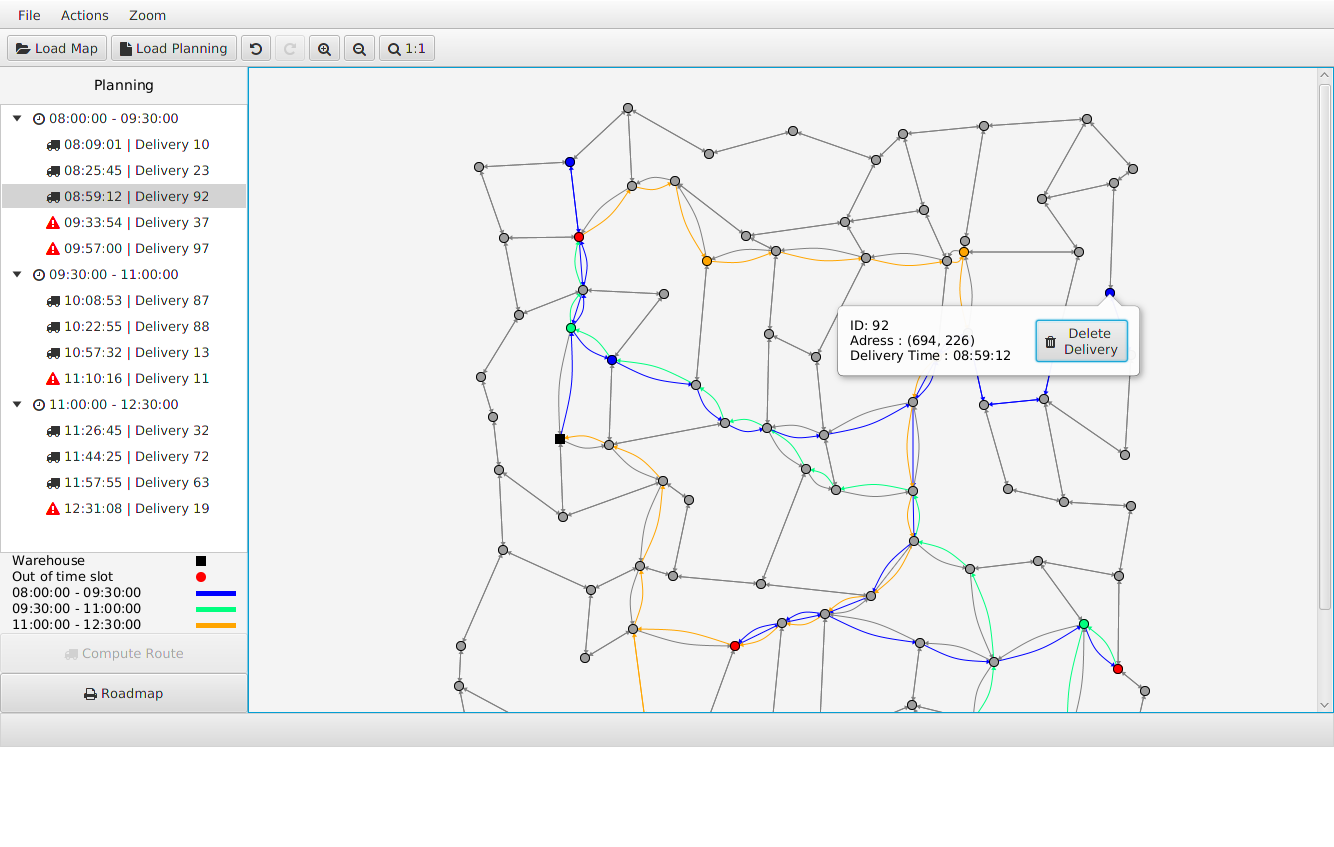
\includegraphics[width=\textwidth]{figures/screenshot.png}}

\noindent\makebox[\textwidth]{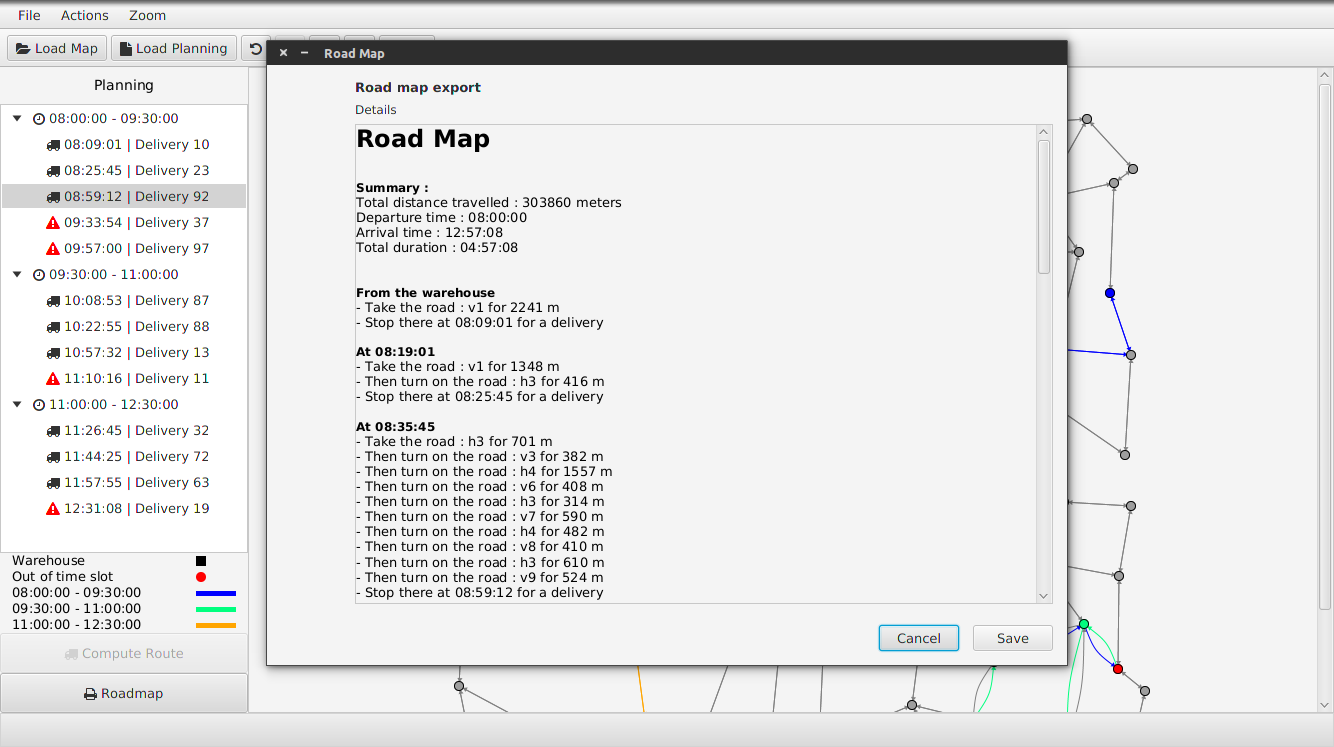
\includegraphics[width=\textwidth]{figures/screenshot-1.png}}
\caption{Captures d'écran du logiciel}

\end{figure}




%%%%%%%%%%%%%%%%%%%%%%%%%%%%%%%%%%%%%%%%% Capture et analyse des besoins

\part{Capture et analyse des besoins}
\label{part:capture-et-analyse-des-besoins}
\setcounter{section}{0}

\section{Planning prévisionnel du projet \it{(FR)}}
\label{sec:planning-previsionnel-du-projet}

Voici le diagramme de Gantt du déroulement du projet.
Nous avions estimé que le projet devait être bien avancé pendant les vacances de la semaine 44 et finaliser les détails durant la semaine 45 ne sachant pas la date initiale du rendu. Bien entendu nous avons étendu la phase d'implémentation une fois cet élément manquant acquis (cf. diagramme de Gantt réel~\ref{sec:planning-effectif-du-projet}).

\begin{figure}[H]
\centering
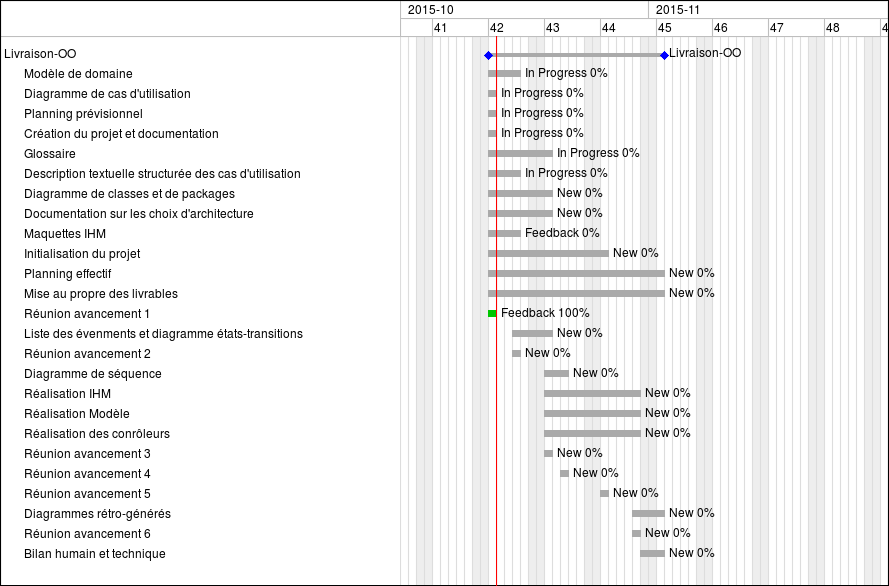
\includegraphics[scale=0.5,angle=0]{redmine/gantt-prev.png}
\caption{Planning prévisionnel}
\end{figure}

Voici la répartition globale des tâches ainsi qu'une rapide estimation des temps pour chacune d'elles afin d'avoir un retour plus conséquent en fin de projet sur le planning prévisionnel.

\begin{figure}[H]
\begin{center}
\begin{tabular}{  l  l  l  }
  \hline
  \bf{Tâche} & \bf{Affectation} & \bf{Temps estimé} \\
  \hline
  %%%% Gestion de projet
  \hline
  \bfit{Gestion de projet} & \multicolumn{2}{r}{\it{Sous-Total : 41 heures}} \\
  \hline
  Création du projet et documentation & Hugues & 3 heures \\
  \hline
  Initialisation du projet & Tous & 2 heures \\
  \hline
  Réunion d'avancement 1 & Antoine & 3,5 heures \\
  \hline
  Réunion d'avancement 2 & Antoine & 3,5 heures \\
  \hline
  Réunion d'avancement 3 & Antoine & 3,5 heures \\
  \hline
  Réunion d'avancement 4 & Antoine & 3,5 heures \\
  \hline
  Réunion d'avancement 5 & Antoine & 3,5 heures \\
  \hline
  Réunion d'avancement 6 & Antoine & 3,5 heures \\
  \hline
  Finalisation des livrables & Tous & 15 heures \\
  \hline
  %%%% Analyse des besoins
  \hline
  \bfit{Analyse des besoins} & \multicolumn{2}{r}{\it{Sous-Total : 18,5 heures}} \\
  \hline
  Modèle de domaine & Estelle, Lisa et Paul & 9 heures \\
  \hline
  Diagramme de cas d'utilisation & Guillaume, Pierre & 2 heures \\
  \hline
  Planning prévisionnel & Antoine & 2 heures \\
  \hline
  Glossaire & Paul, Estelle, Lisa & 1,5 heure \\
  \hline
  Description textuelle structurée des cas d'utilisation & Pierre, Guillaume & 4 heures \\
  \hline
  %%%% Conception
  \hline
  \bfit{Conception} & \multicolumn{2}{r}{\it{Sous-Total : 25 heures}} \\
  \hline
  Liste des évenments et diagramme états-transitions & Estelle, Guillaume et Antoine & 6 heures \\
  \hline
  Diagramme de classes et de packages & Pierre, Paul, Hugues & 12 heures \\
  \hline
  Documentation choix architecture & Paul, Hugues & 3 heures \\
  \hline
  Maquettes IHM & Lisa et Hugues & 2 heures \\
  \hline
  Diagramme de séquence & Pierre & 2 heures \\
  \hline
  %%%% Implémentation et tests
  \hline
  \bfit{Implémentation et tests} & \multicolumn{2}{r}{\it{Sous-Total : 52 heures}} \\
  \hline
  Réalisation IHM & Hugues & 20 heures \\
  \hline
  Réalisation Modèle & Pierre, Lisa et Guillaume & 15 heures \\
  \hline
  Réalisation des contrôleurs & Estelle, Paul et Antoine & 15 heures \\
  \hline
  Diagramme rétro-générés & Antoine & 2 heures \\
  \hline
  %%%% Bilan
  \hline
  \bfit{Bilan} & \multicolumn{2}{r}{\it{Sous-Total : 6 heures}} \\
  \hline
  Planning effectif & Antoine & 2 heures \\
  \hline
  Bilan humain et technique & Antoine & 4 heures \\
  \hline
  %%%% Total
  \hline
  \multicolumn{3}{r}{\bf{Total temps estimé :} 142,5 heures} \\
  \hline
\end{tabular}
\end{center}
\caption{Affectations et estimations des tâches}
\end{figure}

Un certain nombre de tâches supplémentaires sont arrivé ensuite ainsi qu'un redécoupage en sous-tâches pour l'implémentation. Donc le temps estimé a été augmenté une fois que nous avions une vision plus complète sur le travail à effectuer (analyse des besoins et conception terminées).

\section{Domain model \it{(EN)}}
\label{sec:domain-model}

\Todo{We should add a comment here}

\begin{figure}[H]
\centering
\noindent\makebox[\textwidth]{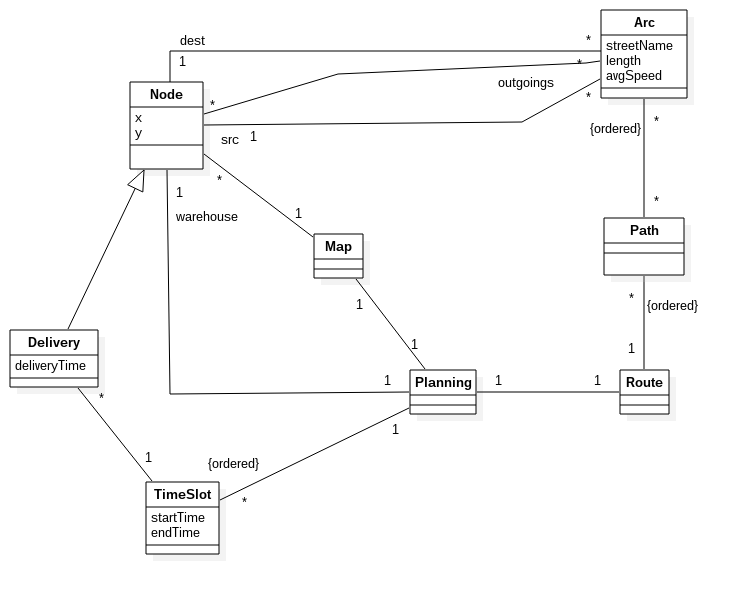
\includegraphics[width=\textwidth]{figures/domain-model.png}}
\caption{Domain Model}
\end{figure}

\section{Glossary \it{(EN)}}
\label{sec:glossary}

Syntax used :
\begin{itemize}
	\item[\textbullet] \bf{Object} \it{(french equivalent)} : definition \\
\end{itemize}

Glossary : 
\begin{itemize}
	\item[\textbullet] \bf{Arc} \it{(tronçon)} : section of road between two intersections described by a street name, an average speed, a length and the id of the destination intersection.
	\item[\textbullet] \bf{Node} \it{(intersection)} : Intersection between two or more arcs (cf. Arc) described by its coordinates and an id.
	\item[\textbullet] \bf{Path} \it{(chemin)} : Ordered list of arcs between two delivery nodes, representing the shortest travel duration.
	\item[\textbullet] \bf{Map} \it{(plan)} : Set of arcs (cf. Arc) and intersections (cf. Node)
	\item[\textbullet] \bf{Delivery} \it{(livraison)} : Special node which must be contained by the final route.
	\item[\textbullet] \bf{Planning} : Set of intersections (cf. Node) to be processed by the route computation algorithm (cf. Route).
	\item[\textbullet] \bf{Route} \it{(tournée)} : Ordered list of paths to travel along (cf. Planning). 
	\item[\textbullet] \bf{TimeSlot} \it{(fenêtre de livraison)} : time interval bounded by a start time and an end time containing a set of deliveries to be honored.
	\item[\textbullet] \bf{Warehouse} \it{(entrepot)} : Special intersection representing both the start and the end point of the route (cf. Route).
	\item[\textbullet] \bf{Average Speed} \it{(vitesse moyenne)} : average speed of vehicles in meters per second on an arc (cf. Arc).
	\item[\textbullet] \bf{Planning File} \it{(fichier de planning)} : XML formated input file, describing a planning (cf. Planning).
	\item[\textbullet] \bf{Map File} \it{(fichier de plan)} : XML formated input file, describing a Map.
	\item[\textbullet] \bf{Route File} \it{(fichier d’itinéraire)} : text formated output file, describing paths to travel along.
\end{itemize}

\section{Use case diagram \it{(EN)}}
\label{sec:use-case-diagram}

\Todo{We should add a comment here}

\begin{figure}[H]
\centering
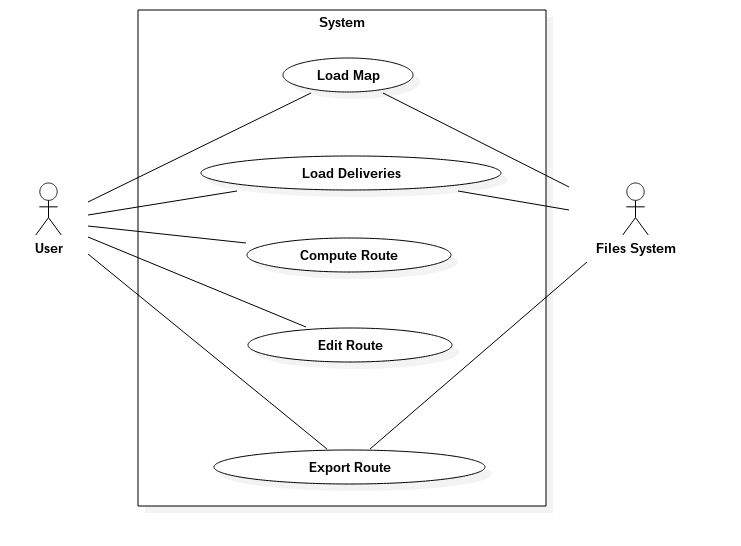
\includegraphics[scale=0.5,angle=0]{figures/use-case.png}
\caption{Use case diagram}
\end{figure}

\section{Structured textual description of use cases \it{(EN)}}
\label{sec:structured-textual-description-of-use-cases}

\subsection{Textual description of \it{Load map}}
\label{subsec:textual-description-of-load-map}

\textbf{Short description :} The user selects an XML file describing a city map. The map is loaded and displayed on the screen.

\textbf{Organized description :}

\begin{itemize}
  \item[•] \textbf{Precondition :} none.
  \item[•] \textbf{Main scenario :}
  \begin{enumerate}
    \item The user indicates that he wants to load a map
    \item The system opens a dialog box allowing the user to select a file.
    \item The user selects the XML file describing the map that he wants to load in the program.
    \item The system interprets the XML file, loads the city map and display the map on the screen.
    \item The user can’t cancel his former modifications anymore.
  \end{enumerate}
  \item[•] \textbf{Alternative scenarios :}
  \begin{itemize}
    \item[3.] The users indicates that he wants to stop the selection of a city map.
    \begin{itemize}
      \item[•] Le system stops the selection and ends the scenario.
    \end{itemize}
    \item[4a.] The XML file selected is incorrect (cf. XML Errors Lists~\ref{subsec:xml-errors-lists}) and doesn’t define a city map.
    \begin{itemize}
      \item[•] The system indicates that the file is incorrect and can’t be loaded, and end the scenario.
    \end{itemize}
    \item[4b.] The opening and the reading of the XML file is denied (cf. IO Errors Lists~\ref{subsec:io-errors-list}).
    \begin{itemize}
      \item[•] The system displays that the loading has failed and indicates the cause (insufficient privileges…) and ends the scenario.
    \end{itemize}
  \end{itemize}
\end{itemize}

\subsection{Textual description of \it{Load delivery request}}
\label{subsec:textual-description-of-load-delivery-request}

\textbf{Short description :} The user selects an XML file describing delivery requests. The system displays the position of each delivery request on the city map.

\textbf{Organized description :}

\begin{itemize}
  \item[•] \textbf{Precondition :} a city map has to be loaded.
  \item[•] \textbf{Main scenario :}
  \begin{enumerate}
    \item The user indicates that he wants to load a delivery request.
    \item The system asks the user to select an XML file in the file system.
    \item The user selects an XML file.
    \item The system interprets the XML file and loads delivery requests, then it deletes the modifications history and displays the delivery points on the city map.
  \end{enumerate}
  \item[•] \textbf{Alternative scenarios :}
  \begin{itemize}
    \item[3.] The user indicates that he wants to stop the selection of the delivery requests.
    \begin{itemize}
      \item[•] The system stops the selection and ends the scenario.
    \end{itemize}
    \item[4a.] The XML file selected is incorrect (cf. XML Errors list~\ref{subsec:xml-errors-lists}) and doesn’t define delivery requests.
    \begin{itemize}
      \item[•] The system indicates that the file is incorrect and can’t be loaded, then it ends the scenario.
    \end{itemize}
    \item[4b.] The opening and the reading of the XML file is denied (cf. IO Errors Lists~\ref{subsec:io-errors-list}).
    \begin{itemize}
      \item[•] The system displays that the generation has failed and indicates the cause (insufficient privileges…) and ends the scenario.
    \end{itemize}
  \end{itemize}
\end{itemize}

\subsection{Textual description of \it{Compute a route}}
\label{subsec:textual-description-of-compute-a-route}

\textbf{Short description :} The users asks the system to compute a route. The route computed by the system is displayed on the screen, as the list of deliveries.

\textbf{Organized description :}

\begin{itemize}
  \item[•] \textbf{Precondition :} a file of delivery requests has to be loaded.
  \item[•] \textbf{Main scenario :}
  \begin{enumerate}
    \item The users asks the system to compute the route.
    \item The system computes the path of the route and displays it on the city map, indicating deliveries that will be late (out of the planned time slot). The system also displays the list of deliveries, in the order of the route, with the time slot and the hour estimated of each delivery.
  \end{enumerate}
  \item[•] \textbf{Alternative scenarios :}
  \begin{itemize}
    \item[1-2.] The user indicates to the system that he wants to interrupt the computing of the route.
    \begin{itemize}
      \item[•] The systems interrupts the computing and ends the scenario.
    \end{itemize}
  \end{itemize}
\end{itemize}

\subsection{Textual description of \it{Add a delivery}}
\label{subsec:textual-description-of-add-a-delivery}

\textbf{Short description :} The user adds a delivery to the route, at a node that isn’t already a delivery point.

\textbf{Organized description :}

\begin{itemize}
  \item[•] \textbf{Precondition :} a route has to be computed.
  \item[•] \textbf{Main scenario :}
  \begin{enumerate}
    \item The user indicates that he wants to add a delivery to the route.
    \item The system asks the user to select an empty node, where the delivery will be added.
    \item The user selects the node where the delivery will be executed.
    \item The system asks the user to select the delivery that will be executed before the one he wants to add.
    \item The user selects the delivery that will be executed before the one he wants to add.
    \item The system selects a default time slot (the same time slot as the one of the delivery that will be executed before the new one).
    \item The user confirms the new delivery request.
    \item The system adds the new delivery, updates the path between the previous point and the next point and refreshes the displaying of the map and the route. The delivery times are also reloaded.
  \end{enumerate}
  \item[•] \textbf{Alternative scenarios :}
  \begin{itemize}
    \item[2.] The user selects a node that is already a delivery point.
    \begin{itemize}
      \item[•] The system displays an error message and ends the scenario.
    \end{itemize}
    \item[6.] The user selects another time slot than the one which is selected by default, in the list of the time slots that already exists.
    \begin{itemize}
      \item[•] The system takes the time slot chosen by the user and goes to the step 7.
    \end{itemize}
    \item[1-7.] The user interrupts his request.
    \begin{itemize}
      \item[•] The request isn’t taken into account and the system ends the scenario.
    \end{itemize}
  \end{itemize}
\end{itemize}

\subsection{Textual description of \it{Delete a delivery}}
\label{subsec:textual-description-of-delete-a-delivery}

\textbf{Short description :} The user deletes an existing delivery of the route.

\textbf{Organized description :}

\begin{itemize}
  \item[•] \textbf{Precondition :} a route has to be computed.
  \item[•] \textbf{Main scenario :}
  \begin{enumerate}
    \item The user selects a delivery and indicates that he wants to delete it.
    \item The system shows a deletion confirmation.
    \item The user confirms the deletion.
    \item The system deletes the delivery, updates the path between the previous delivery and the next one and displays the new route.
  \end{enumerate}
  \item[•] \textbf{Alternative scenarios :}
  \begin{itemize}
    \item[3.] The user cancels his deletion request.
    \begin{itemize}
      \item[•] The deletion request isn’t taken into account and the system ends the scenario.
    \end{itemize}
  \end{itemize}
\end{itemize}

\subsection{Textual description of \it{Swap two deliveries}}
\label{subsec:textual-description-of-swap-two-deliveries}

\textbf{Short description :} The user swaps two deliveries.

\textbf{Organized description :}

\begin{itemize}
  \item[•] \textbf{Precondition :} a route has to be computed.
  \item[•] \textbf{Main scenario :}
  \begin{enumerate}
    \item The user moves graphically the delivery on another delivery. If the delivery time of the selected delivery is lower (respectively higher) than the delivery time of the second one, then the second delivery has to be executed before (respectively after) the first one.
    \item The system updates the path of the route and displays it.
  \end{enumerate}
  \item[•] \textbf{Alternative scenarios :}
  \begin{itemize}
    \item[1-2.] The user interrupts his swap request.
    \begin{itemize}
      \item[•] The swap request isn’t taken into account and the system ends the scenario.
    \end{itemize}
    \item[2a.]  The user drop the delivery to move on the same node where it was before, or on an area that isn’t a delivery node.
    \begin{itemize}
      \item[•] The system ignores the swap and ends the scenario.
    \end{itemize}
  \end{itemize}
\end{itemize}

\subsection{Textual description of \it{Generate an itinerary}}
\label{subsec:textual-description-of-generate-an-itinerary}

\textbf{Short description :} The user asks the system to generate an itinerary.

\textbf{Organized description :}

\begin{itemize}
  \item[•] \textbf{Precondition :} a route has to be computed.
  \item[•] \textbf{Main scenario :}
  \begin{enumerate}
    \item The user indicates that he wants to generate an itinerary.
    \item The system asks the user to name the file and to select the location where it will be saved.
    \item The user names the file and selects a location.
    \item The system generates an itinerary in txt format, with the list of the deliveries, and displays a message on the screen when it’s done.
  \end{enumerate}
  \item[•] \textbf{Alternative scenarios :}
  \begin{itemize}
    \item[3.] The user indicates that he wants to interrupt the generation.
    \begin{itemize}
      \item[•] The system stops the generation and ends the scenario.
    \end{itemize}
    \item[4.]  The record is denied.
    \begin{itemize}
      \item[•] The system displays that the generation failed and indicates the cause (insufficient privileges…) and ends the scenario.
    \end{itemize}
  \end{itemize}
\end{itemize}

\subsection{Alternative scenarios that can occur at any moment}
\label{subsec:alternative-scenarios-that-can-occur-at-any-moment}

\begin{itemize}
  \item[a.] The user chooses to cancel his last modification.
  \begin{itemize}
    \item[•] The system cancels the last modification if it exists and restores the previous route.
  \end{itemize}
  \item[b.] The users chooses to redo a cancelled modification.
  \begin{itemize}
    \item[•] The system redoes the last cancelled modification if it exists, and restores the corresponding route.
  \end{itemize}
\end{itemize}

%%%%%%%%%%%%%%%%%%%%%%%%%%%%%%%%%%%%%%%%%%%%%%%%%%%%%%%%%%%% Conception
\part{Conception}
\label{part:conception}
\setcounter{section}{0}

\section{User-level events list and State-Transition Diagram \it{(EN)}}
\label{sec:user-level-events-list-and-state-transition-diagram}

\Todo{We should add a comment here}

\bf{The user-level events list :}
\begin{itemize}
  \item[•] \it{btnLoadMap :} the user request to load a new map from a XML file.
  \item[•] \it{btnLoadPlanning :} the user request to load a new planning from a XML file.
  \item[•] \it{btnGenerateRoute :} the event to compute the fastest route to make all deliveries.
  \item[•] \it{btnCancel :} the user request to cancel the current process.
  \item[•] \it{btnValidateFile :} the user request to validate a file selected.
  \item[•] \it{leftClickPressedOnDelivery :} when the user make a left click pressed on a delivery.
  \item[•] \it{leftClickReleased :} when the user releaded the previous left click pressed on a delivery.
  \item[•] \it{clickOnDelivery :} when the user make a simple click on a delivery.
  \item[•] \it{clickSomewhereElse :} when the user click on something not interactive in the application.
  \item[•] \it{clickOnEmptyNode :} when the user mae a simple click on an empty node.
  \item[•] \it{btnAddDelivery :} the user request to add a new delivery on a previous empty node selected.
  \item[•] \it{btnRemoveDelivery :} the user request to remove a delivery previously selected.
  \item[•] \it{clickOnWarehouse :} when the user make a simple click on the warehouse.
  \item[•] \it{btnCloseMap :} the user request to close the current map loaded.
  \item[•] \it{btnClearPlanning :} the user request to close the current planning loaded.
\end{itemize}

\begin{figure}[H]
\noindent\makebox[\textwidth]{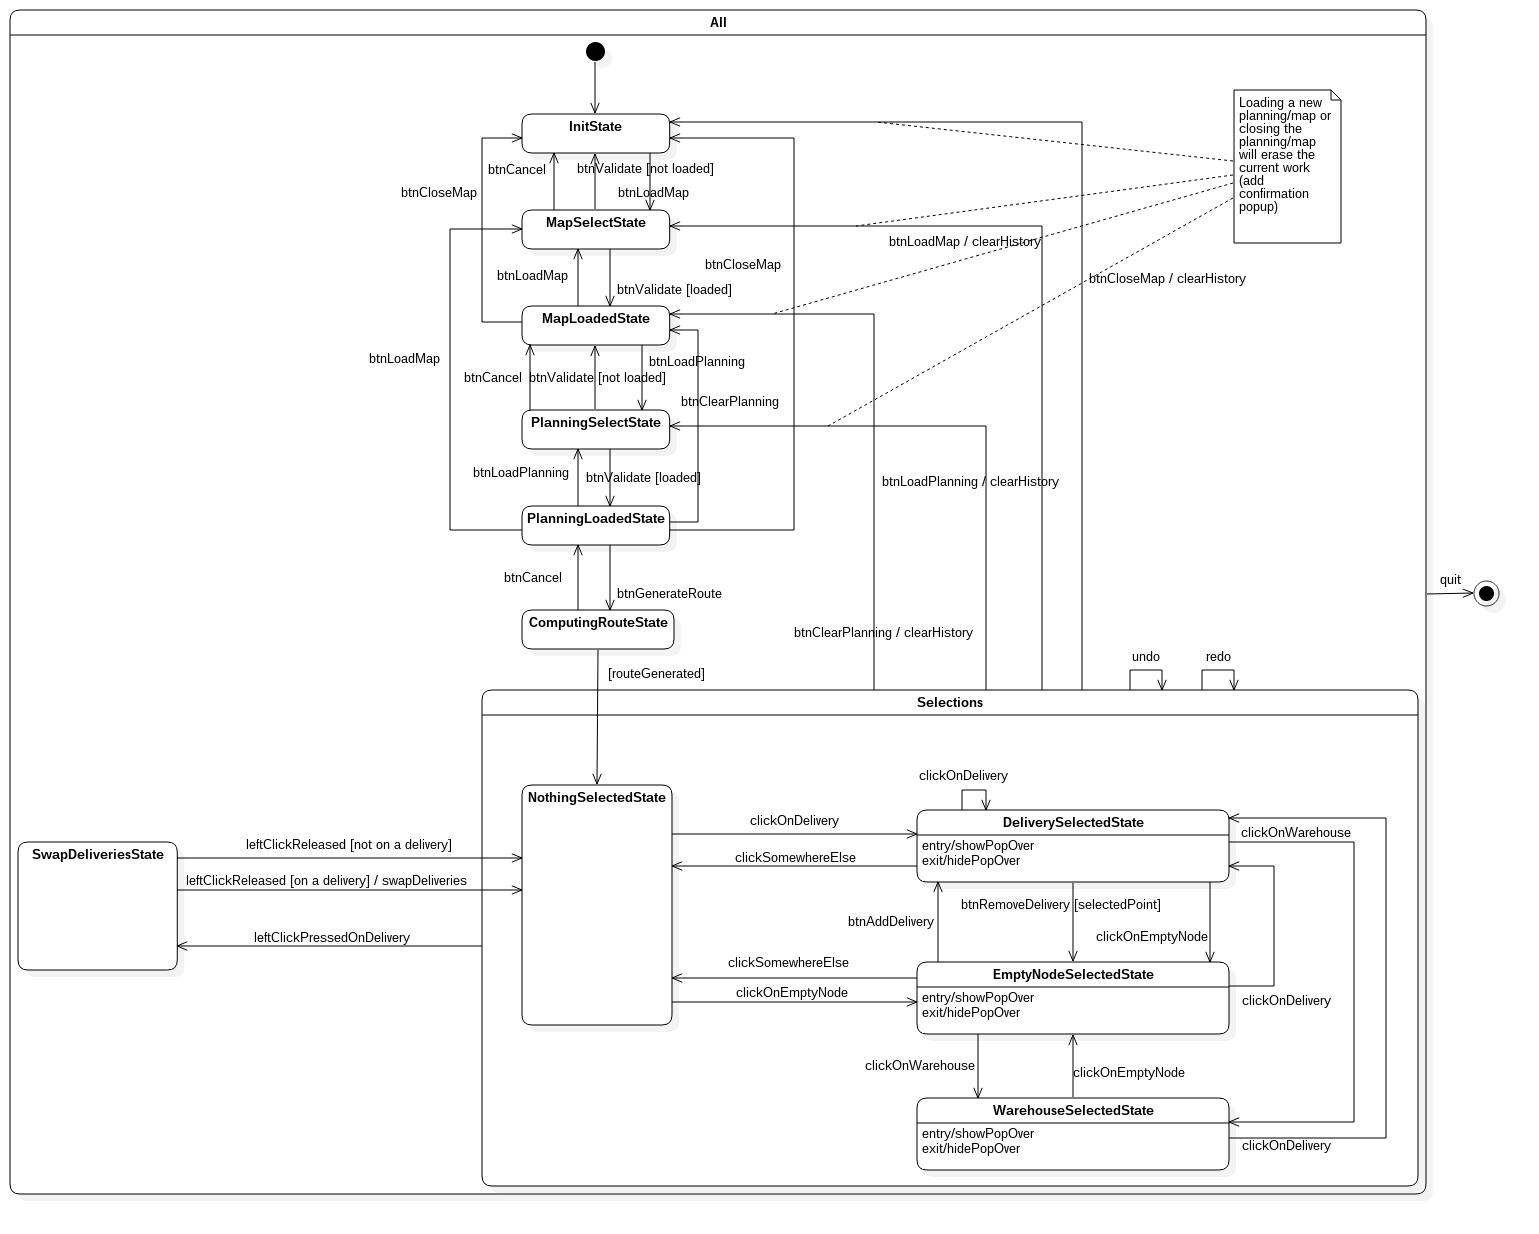
\includegraphics[scale=0.43,angle=90]{figures/state-machine.png}}
\caption{State-Transition Diagram}
\end{figure}

\section{Packages and Classes Diagrams \it{(EN)}}
\label{sec:packages-and-classes-diagrams}

\subsection{Model related diagrams}
\label{subsec:model-related-diagrams}

The following figure shows classes which are part of the model package. These classes implements the Domain Model and others objects needed to properly use design patterns. All methods are not shown, especially getters and setters. Further information are available in III.3 section.

\vspace*{-6.5cm}
\begin{figure}[H]
\centering
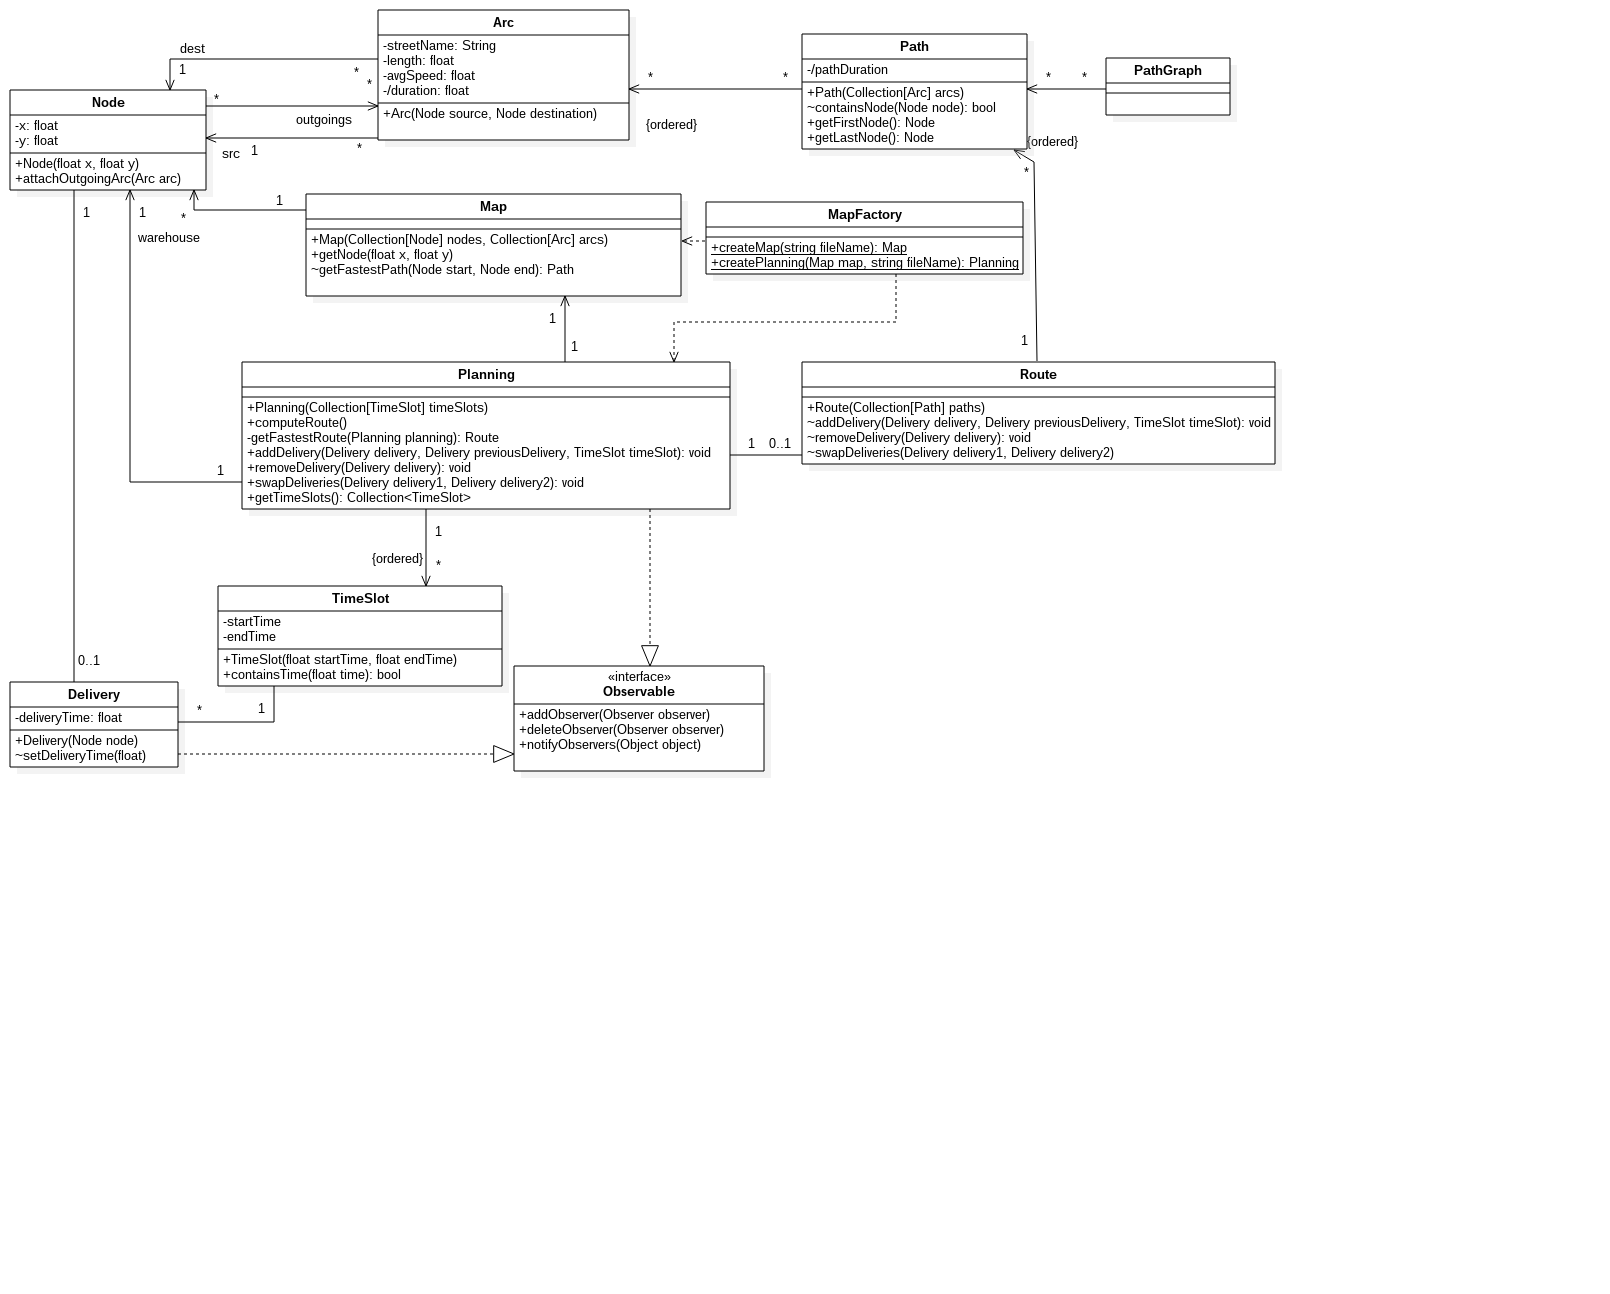
\includegraphics[scale=0.52,angle=90]{figures/model-class.png}
\caption{Model package including classes}
\end{figure}

\subsection{View related diagrams}
\label{subsec:view-related-diagrams}

The following figure presents the view package, it is reduced to objects linked directly or indirectly to the Domain Model. Some objects such as PopOverContent and its derivates exists due to technological choices made to represent information about nodes and the way user will interact with them. UIManager which is part of the controller package but is strongly related to this package as it is in charge of instanciating the MainWindow. Further information are available in III.3 section.

\begin{figure}[H]
\noindent\makebox[\textwidth]{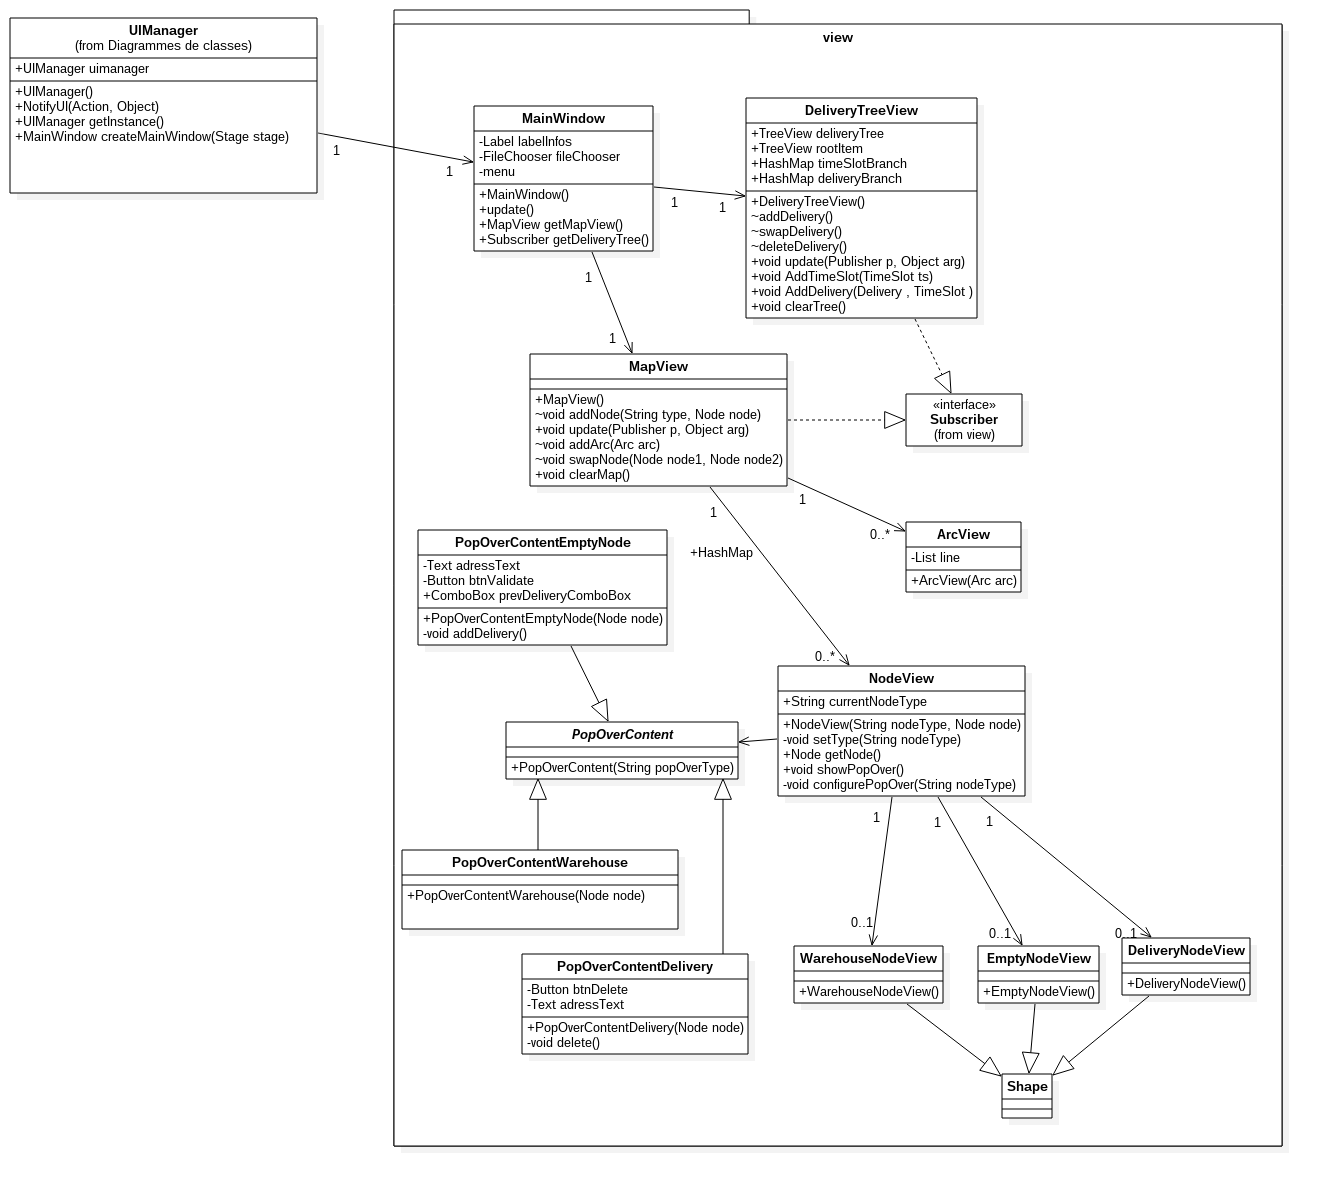
\includegraphics[scale=0.40,angle=0]{figures/view-class.png}}
\caption{View package including classes}
\end{figure}

\subsection{Controller related diagrams}
\label{subsec:controller-related-diagrams}

The three following figures show how we designed the controller. The controller is in fact divided into four Managers which are in reality sub-controllers dedicted to specific tasks. They have been named according to their role. Two more packages, states and commands, have been added to implement State and Command design patterns. These two packages are used by the ContextManager which is charged of assuring application process consistency. Further information are available in III.3 section.  

\begin{figure}[H]
\centering
\noindent\makebox[\textwidth]{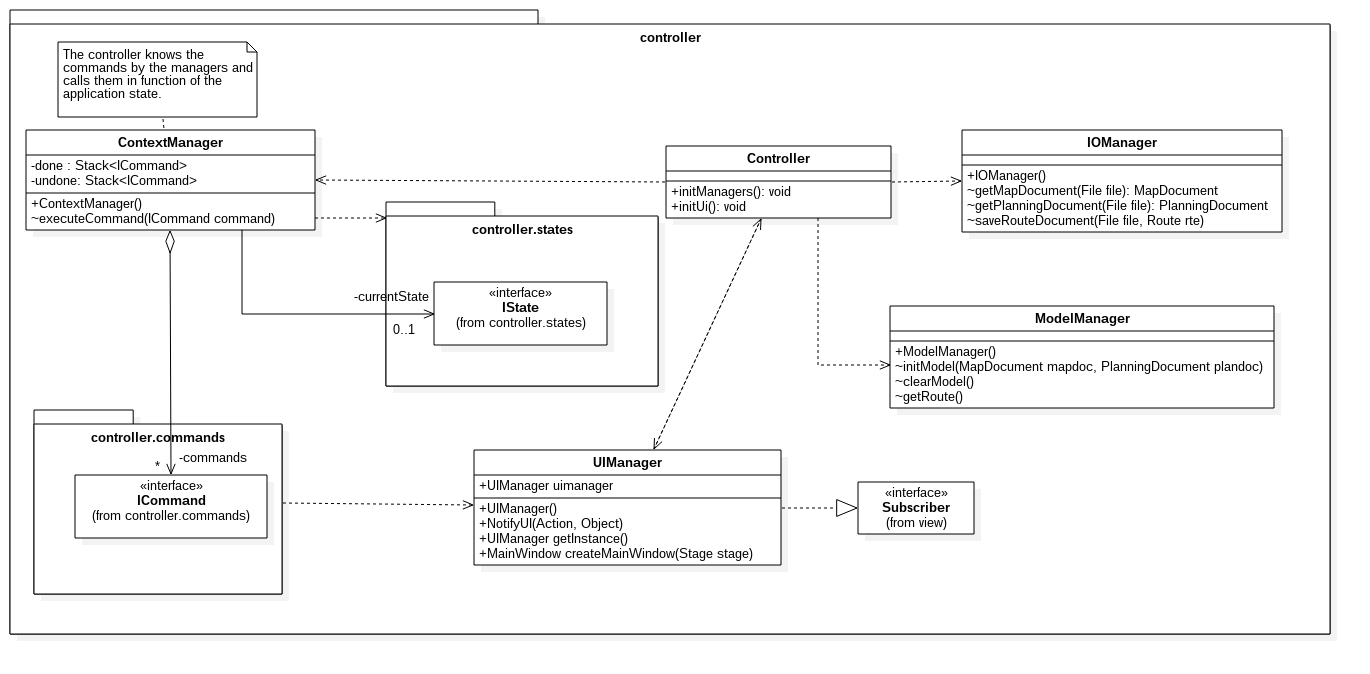
\includegraphics[scale=0.5,angle=90]{figures/controller-class.png}}
\caption{Controller package including classes}
\end{figure}

\begin{figure}[H]
\noindent\makebox[\textwidth]{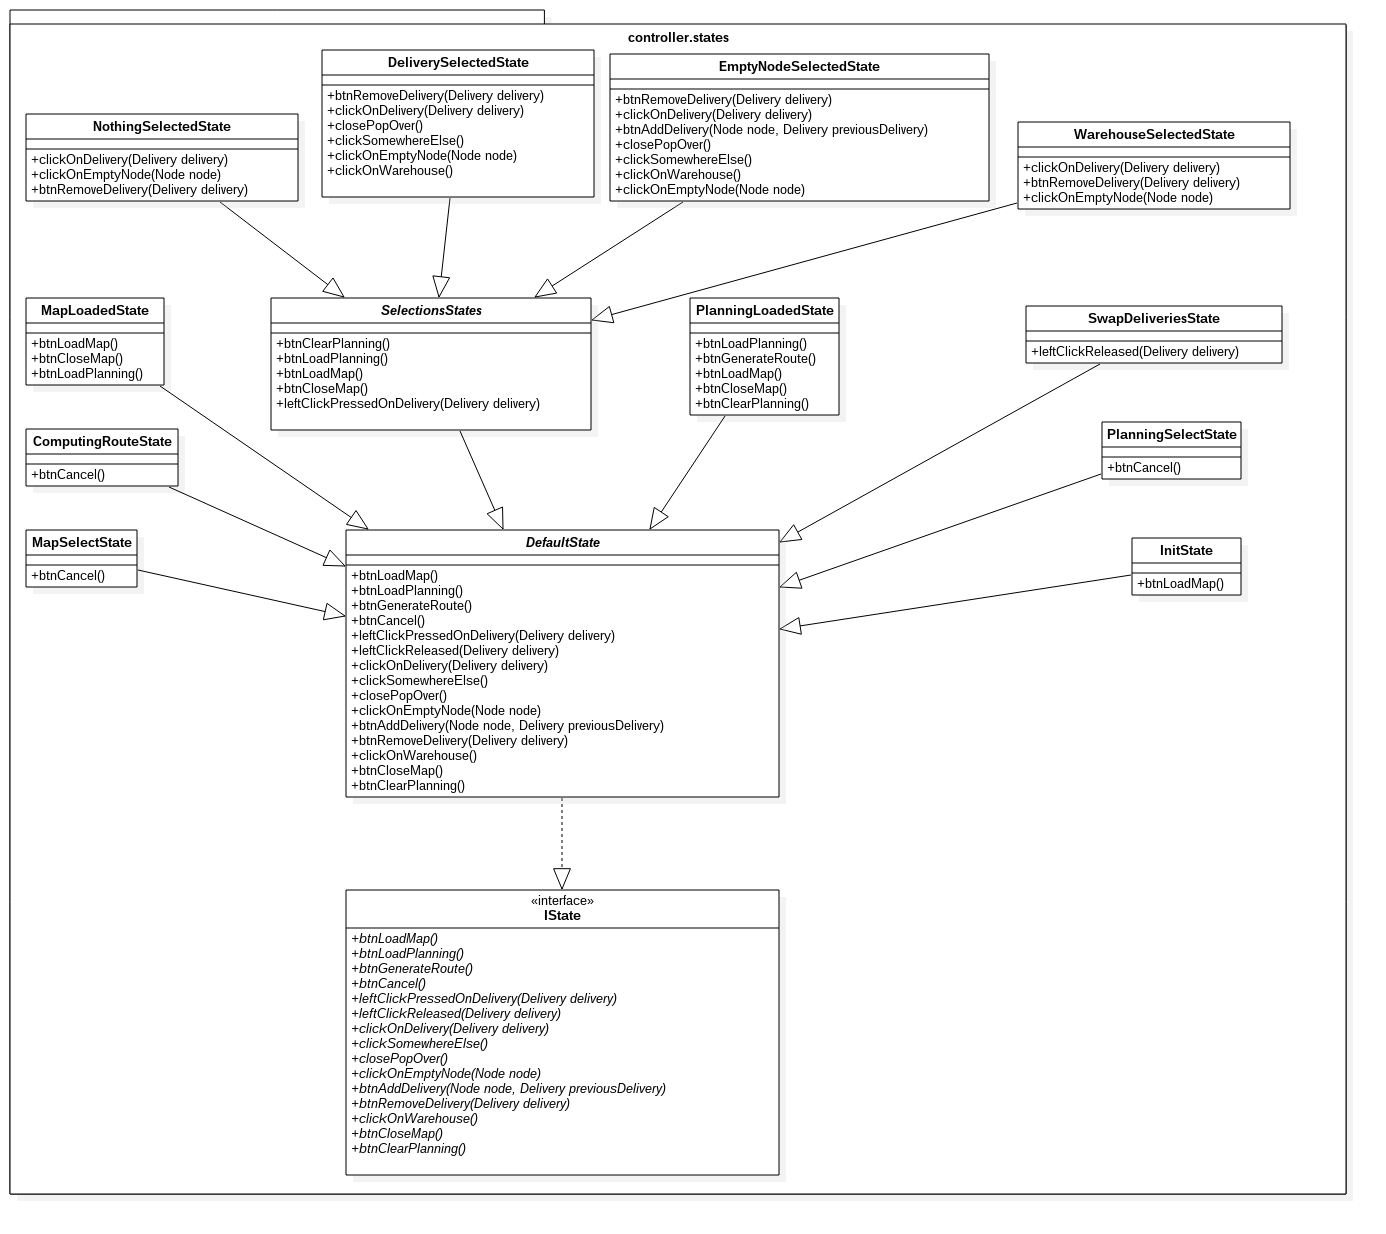
\includegraphics[scale=0.4,angle=0]{figures/controller_states-class.png}}
\caption{Controller States package including classes}
\end{figure}

\begin{figure}[H]
\centering
\noindent\makebox[\textwidth]{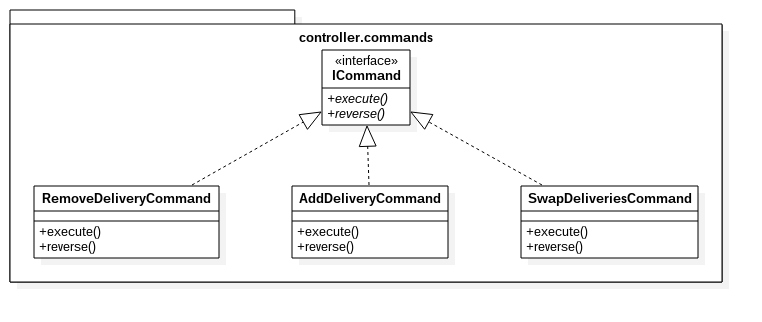
\includegraphics[scale=0.5,angle=0]{figures/controller_commands-class.png}}
\caption{Controller Commands package including classes}
\end{figure}

\subsection{Other diagrams}
\label{subsec:other-diagrams}

The next figure shows utils package which contains all utility classes which can also be called helpers. These objects are used to implement design patterns or - as XML parsers - to provide convenient interfaces to convert data stored in files into objects usable by the application. Further information are available in III.3 section.

\begin{figure}[H]
\centering
\noindent\makebox[\textwidth]{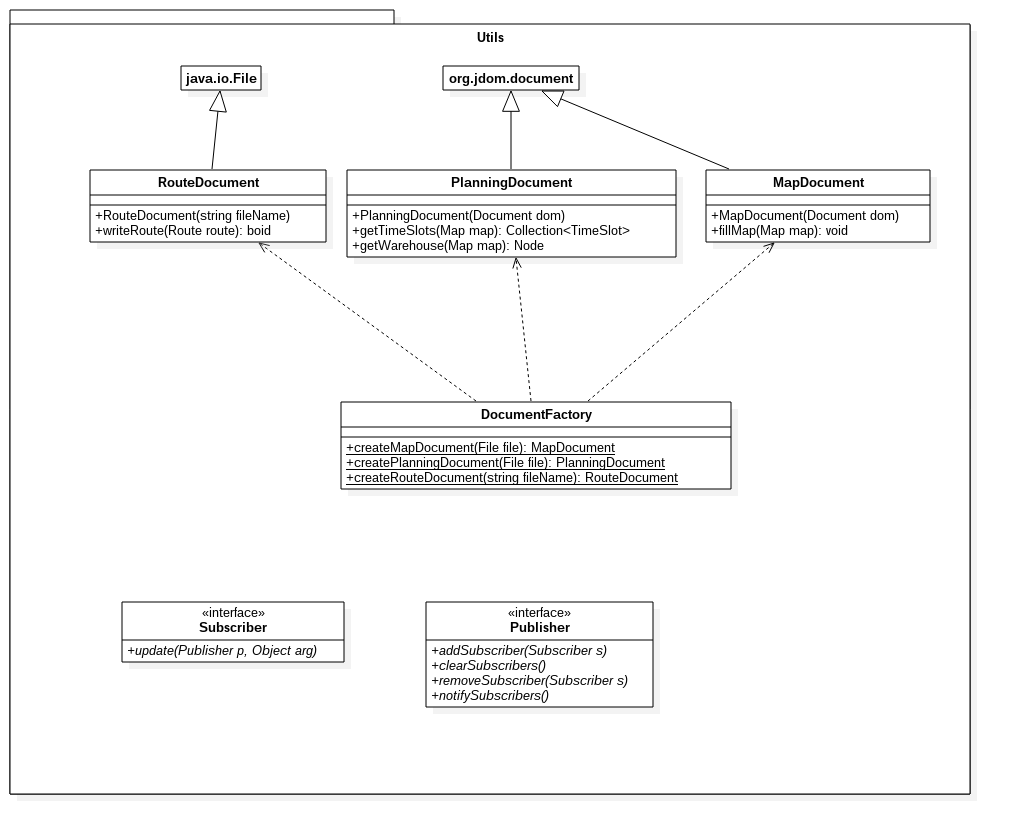
\includegraphics[scale=0.5,angle=0]{figures/utils-class.png}}
\caption{Utils package and its classes}
\end{figure}

\section{Choix architecturaux et patrons de conception utilisés \it{(FR)}}
\label{sec:choix-architecturaux-et-patrons-de-conception-utilises}

\bfit{Les classes cités dans ce document pouvant présenter des ambiguïtés sont référencés dans le glossaire.} \\

Nous choisirons tout d'abord de respecter l'architecture globale de type \bf{MVC} afin de garantir une simplicité de maintenance corrective et évolutive de l'application. Les différents composants appartenant à ces trois grandes catégories (Modèle, Vue et Contrôleur) implémenteront divers patrons de conception. \\

Concernant l'architecture globale, nous avons choisi de faire en sorte que la hiérarchie en couche soit parfaitement respectée, c'est-à-dire que la vue ne modifie en aucun cas le modèle sans  passer par le contrôleur. La vue, cependant, implémente pour certains de ses composants le patron \bf{Observateur} pour détecter les modifications au niveau du modèle et se modifier ou demander au contrôleur d'effectuer des actions en conséquence.\\

Les objets du modèle, qui constitue l'ensemble des données métier manipulées par l'application représentées par des objets, sont pour la plupart des conteneurs de données améliorés et n'implémentent pas de traitements particuliers. Il y a cependant une exception, l'objet \bf{Map} implémente l'algorithme permettant de calculer la tournée et de créer l'objet \bf{Route} correspondant. Certains objets, tels que \bf{Map} et \bf{Planning}, constituent en réalité des conteneurs d'autres objets du modèle. Ces objets agissent comme des \bf{Fabrique}s pour les objets qu'ils contiennent. Cela permet de garantir la cohérence des objets contenus dans ces conteneurs ainsi que la maîtrise de la durée de vie de ces derniers. Comme indiqué dans le paragraphe précédent, le modèle est observé par la vue ce qui signifie que certains objets du modèle sont \bf{Observable}s. Ce mécanisme nous permet de notifier la vue de changements au niveau du modèle. \\

L'objet qui représente la \bf{Map}, \bf{MapView}, ainsi que celui qui représente l'arbre des livraisons implémentent le patron \bf{Observateur}. Pour le reste, la vue est isolée du modèle. Celui peut donc fonctionner indépendamment de la vue.\\

Nous avons ajouté un package supplémentaire n'apparaissant pas dans l'architecture MVC afin d'y placer tous les objets étant catégorisés utilitaires, c'est-à-dire rendant des services aux autres objets de l'application mais dont les traitements auraient pu être intégrés aux objets de l'application si nous n'avions pas fait le choix de segmenter les traitements. Ce package, nommé utils, contient notamment les objets constituant des interfaces plus simples pour la création des objets du modèle possédant une représentation sous forme de fichiers XML. Ce package contient également une classe permettant la conversion de types spéciaux propres à l'application et une \bf{Fabrique} pour les objets d'interface avec les fichiers. \\

Le choix majeur effectué concernant le contrôleur est de séparer les traitements en créant des sous-composants de ce contrôleur principal. Ce package contient donc un ensemble de  contrôleurs spécialisés. Cette organisation au niveau du contrôleur présente de nombreux avantages et notamment la simplification des procédures de gestion des erreurs, leurs causes étant segmentées à l'image des contrôleurs qui peuvent les rencontrer. 
Nous avons donc choisi de dédier un contrôleur à la gestion du modèle, il constitue en réalité l'interface du contrôleur avec le modèle. Ce contrôleur se nomme \bf{ModelManager} et garantie la cohérence du modèle exploité par l'application, tout en proposant une interface simple pour l'accès au modèle. Il ajoute également un niveau d'encapsulation supplémentaire concernant les données manipulées dans le modèle. 

Un second contrôleur, nommé \bf{IOManager}, est chargé des interactions avec le système de fichiers du système d'exploitation exécutant l'application. C’est à son niveau que sont traitées les erreurs de type Entrée/Sortie telles que l'absence de fichier ou encore les privilèges insuffisants pour lire/écrire un fichier. De nouveau, ce contrôleur propose une interface simple pour effectuer les opérations dont il est chargé. 

Ensuite, l'\bf{UIManager}, pendant du \bf{ModelManager}, mais pour l'interface graphique cette fois. Il constitue une interface, simple d'utilisation, entre le contrôleur et la vue. Cela permet de centraliser les informations provenant de la vue. C'est aussi le rôle de ce contrôleur d'interpréter les ordres en provenance de la vue pour les convertir en ordres exécutables par le \bf{ContextManager}. 

Le \bf{ContextManager} a deux rôles majeurs qui lui valent d'implémenter deux patrons de conception qui sont le patron État et le patron Commande. Il a tout d'abord pour rôle d'entretenir la machine à états globale de l'application, c'est-à-dire de garantir à chaque instant qu'une commande utilisateur déclenchera les bons traitements dans l'application et donc les bonnes réactions de l'interface utilisateur et du modèle. Son second rôle est d'entretenir un historique des modifications effectuées de sorte à ce que l'utilisateur puisse défaire et refaire les dernières actions qu'il a effectué. Ce contrôleur assure à l'utilisateur que l'action qu'il veut effectuer a du sens dans le processus global que déroule l'application. Il est dans cette optique étroitement lié à l'\bf{UIManager} qui lui fait parvenir les commandes de l'utilisateur.
Il est, à ce stade, important de préciser que ces différents composants implémentent tous le patron Singleton afin de garantir l'unicité de chaque interface et par conséquent l'unicité du modèle, de l'état de global de l'application et de l'historique des commandes effectuées.

L'objet \bf{Controller} présent dans le package ne constituent en réalité que le point d'entrée de l'application, il est appelé par la procédure main qui l'utilise pour initialiser les différents composants du contrôleur, c'est-à-dire réaliser la première instanciation des composants du contrôleur, puis démarrer l'interface graphique.

On peut également considérer l'\bf{UIManager} et le \bf{ModelManager} comme des \bf{Façade}s respectivement pour la vue et le modèle. 

\Todo{Ajouter des explications concernant les patrons de conception utilisés.}

\section{Sequence Diagram describing Route computation process \it{(EN)}}
\label{sec:sequence-diagram-describing-route-computation-process}

\begin{figure}[H]
\centering
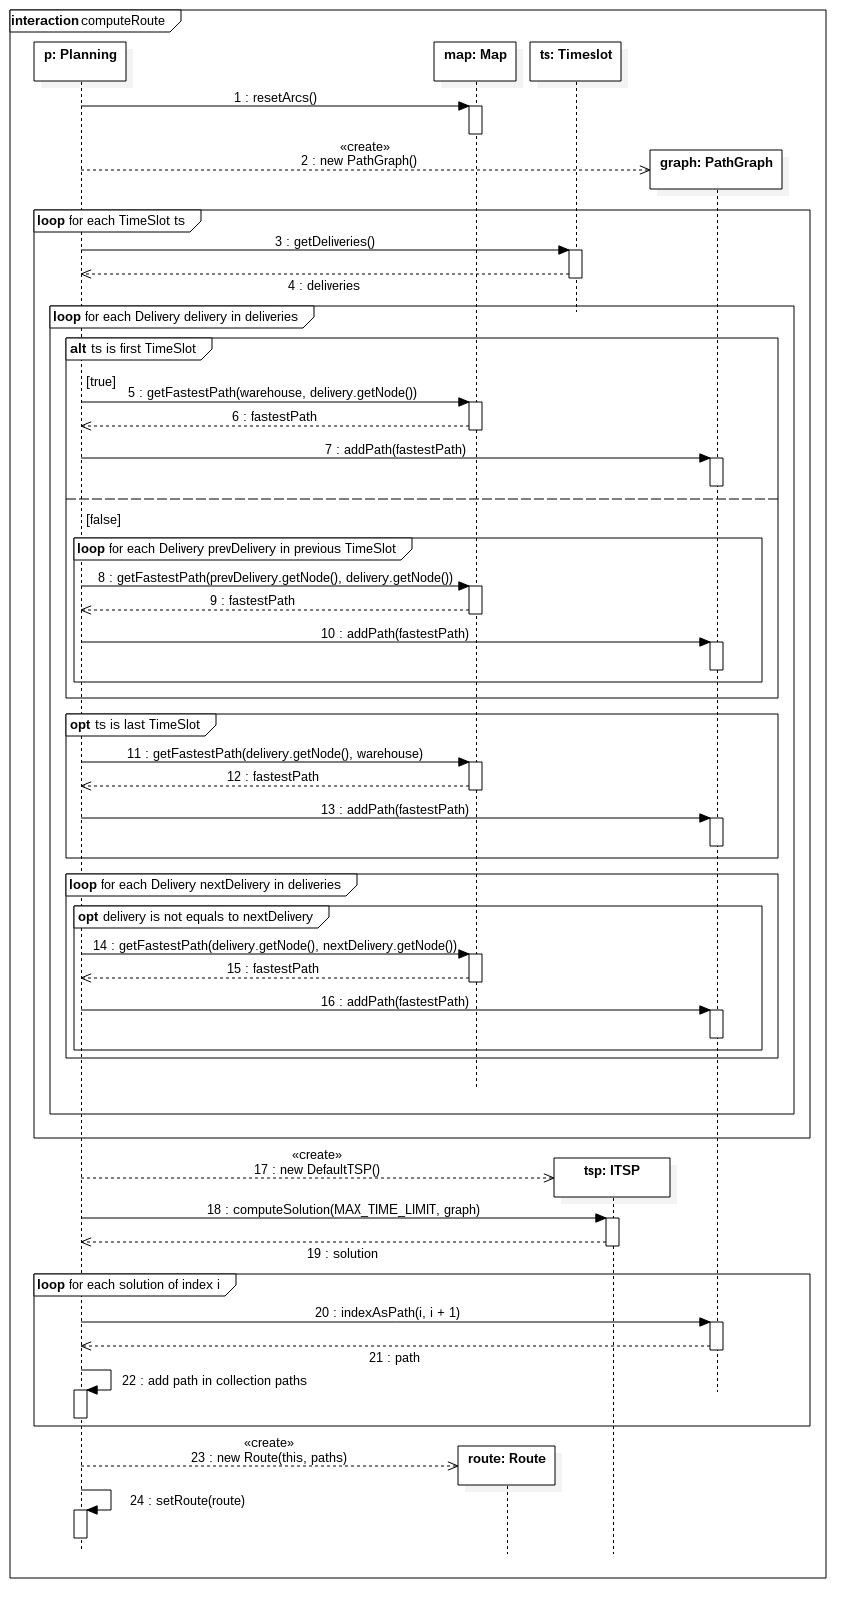
\includegraphics[scale=0.35,angle=0]{figures/sequence-diagram-route-compute.png}
\caption{Sequence diagram describing route computation process}
\end{figure}

\begin{figure}[H]
\centering
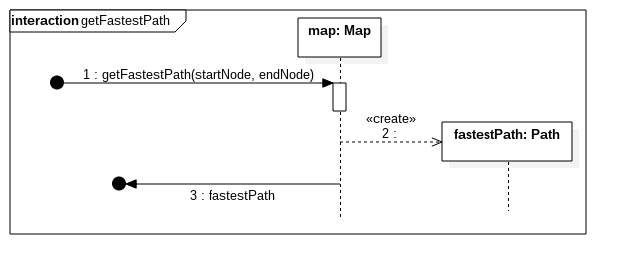
\includegraphics[scale=0.6,angle=0]{figures/sequence-diagram-route-compute-ref-get-fastest-path.png}
\caption{Reference of the sequence diagram : getFastestPath}
\end{figure}

\Todo{We should add a comment here}

%%%%%%%%%%%%%%%%%%%%%%%%%%%%%%%%%%%%%%%%%%%%%%% Implémentation et tests

\part{Implémentation et tests}
\label{part:implementation-et-tests}
\setcounter{section}{0}

\section{Notes related to source code, its documentation and unit tests \it{(EN)}}
\label{sec:notes-related-to-source-code}

\Todo{Add notes here if needed or remove this section}

\section{Packages and classes diagrams generated from source code \it{(EN)}}
\label{sec:packages-and-classes-diagrams-generated-from-source-code}

\Todo{Retro-generated diagrams}

%%%%%%%%%%%%%%%%%%%%%%%%%%%%%%%%%%%%%%%%%%%%%%%%%%%%%%%%%%%%%%%% Bilan

\part{Bilan}
\label{part:bilan}
\setcounter{section}{0}

\section{Planning effectif du projet \it{(FR)}}
\label{sec:planning-effectif-du-projet}

Voici le planning effectif du projet sous forme d'un Gantt. Comme vous pouvez le voir il diffère du prévisionnel avec un grand nombre de tâche supplémentaire et un redécoupage en sous-tâche.

\begin{figure}[H]
\centering
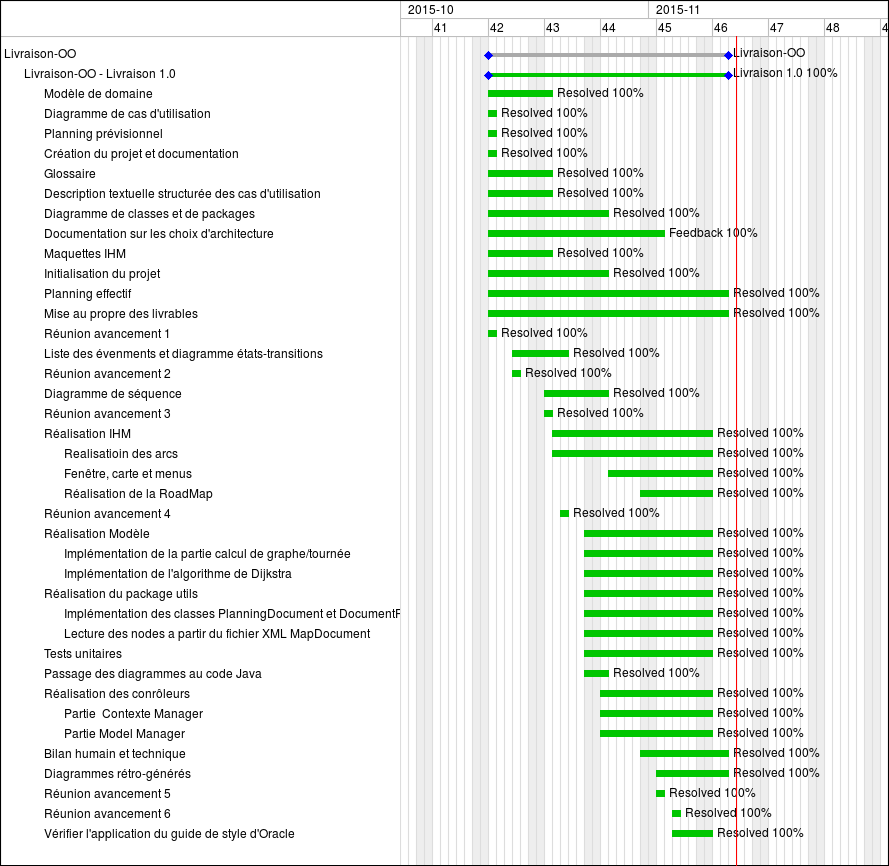
\includegraphics[scale=0.5,angle=0]{redmine/gantt-real.png}
\caption{Planning effectif}
\end{figure}

\section{Temps passés sur les tâches \it{(FR)}}
\label{sec:temps-passes-sur-les-taches}

Le suivi de projet a été fait en utilisant l'outil Redmine. Vous trouverez en annexe (cf. \ref{sec:cr-des-taches-redmine}~Compte-rendu des tâches) un aperçu des temps assignations et des temps passés pour chaque tâche. L'affectation correspond à la personne en charge de cette tâche, cela ne veut pas dire que les autres membres de l'hexanome n'ont pas travaillé dessus.

Voici le détails des heures effectués pour chaque personne :

\begin{figure}[H]
\centering
\pgfplotstabletypeset[
    col sep=semicolon,
    string type,
    columns={Utilisateur,Temps total},
    columns/Utilisateur/.style={column name=Utilisateur, column type={|l}},
    columns/Temps total/.style={column name=Temps Total (heures), column type={|r|}},
    every head row/.style={before row=\hline,after row=\hline},
    every last row/.style={before row=\hline,after row=\hline},
    ]{redmine/users-time.csv}
\caption{Temps passés par personne}
\end{figure}

Vous trouverez en annexe le détail par demande des temps passés (cf. \ref{sec:details-des-temps-passes}~Détail des temps passés) ainsi que le détail par tâche (cf. \ref{sec:cr-des-taches-redmine}~Compte-rendu des tâches).

\section{Bilan humain et technique \it{(FR)}}
\label{sec:bilan-humain-et-technique}

\subsection{Dépassements des estimations}
\label{subsec:depassements-des-estimations}

\Todo{Rédiger une synthèse ici}

\subsection{Bilan humain et ressentis des membres}
\label{subsec:bilan-humain}

\Todo{Rédiger une synthèse ici}

\subsection{Bilan technique}
\label{subsec:bilan-technique}

\subsection{Synthèse}
\label{subsec:synthese}

%%%%%%%%%%%%%%%%%%%%%%%%%%%%%%%%%%%%%%%%%%%%%%%%%%%%%%%%%%%%%%%% Annexes

\part{Annexes}
\label{part:annexes}
\setcounter{section}{0}

\section{Errors lists \it{(EN)}}
\label{sec:errors-lists}


\subsection{IO Errors List}
\label{subsec:io-errors-list}

This section presents a list of errors which can occur during Input/Output operations such as reading or writing files. \\

\textbf{Input errors :}
\begin{itemize}
  \item[•] \textbf{Cant Read File Error :} the folder is not readable, user’s privileges doesn’t match required privileges.
  \item[•] \textbf{Missing File Error :} the file is missing in the OS File System. \\
\end{itemize}

\textbf{Output errors :}
\begin{itemize}
  \item[•] Cant Write File Error : the folder is not writable, user’s privileges don’t match required privileges.  
\end{itemize}

\subsection{XML errors list}
\label{subsec:xml-errors-lists}

The following lists presents all errors which can be found when reading input XML files.\\

This list contains errors shared by both map definition file and planning definition file.\\

\textbf{Shared errors:}
\begin{itemize}
  \item[•] \textbf{Syntax errors :}
  \begin{itemize}
    \item[•] \textbf{Unexpected End Of File Error :} XML file is not well formatted, tags are not closed properly.\\
  \end{itemize}
\end{itemize}

The next list contains all semantic errors that can occur when parsing XML data. Errors are sorted by file.\\ 

\textbf{File specific errors :}
\begin{itemize}
  \item[•] \textbf{Semantic errors :}
  \begin{itemize}
    \item[•] \textbf{Map file :}
    \begin{itemize}
      \item[•] \textbf{Empty Map Error :} root tag has no child.
      \item[•] \textbf{Missing Node Attribute :} missing id, x or y attribute.
      \item[•] \textbf{Empty Node Error :} tag Node has no outgoing arc.
      \item[•] \textbf{Duplicate Node ID Error :} two or more nodes share the same ID.
      \item[•] \textbf{Duplicate Node Error :} two or more nodes share the same coordinates.
      \item[•] \textbf{Duplicate Arc Error :} two or more outgoing arcs of a single node share the same destination node. 
      \item[•] \textbf{Missing Destination Node Error :} the node referenced by an arc as its destination doesn’t exist. 
      \item[•] \textbf{Invalid Average Speed Value Error :} an arc specified average speed is missing, negative or zero. 
      \item[•] \textbf{Invalid Length Value Error :} an arc specified length is missing, negative or zero.
    \end{itemize}

    \item[•] \textbf{Planning file :}
    \begin{itemize}
      \item[•] \textbf{Missing Warehouse Error :} warehouse tag is missing or the id of the specified warehouse doesn’t match any of the node in the Map.
      \item[•] \textbf{Duplicate Warehouse Error :} more than one warehouse tag is present in the input file.
      \item[•] \textbf{Missing TimeSlot Error :} the file doesn’t specify a timeslot.
      \item[•] \textbf{Duplicate TimeSlot Error :} two or more timeslots have the same start time and end time.
      \item[•] \textbf{Null TimeSlot Error :} a timeslot has the same start and end time.
      \item[•] \textbf{Intersecting TimeSlot Error :} two or more timeslots are intersecting.
      \item[•] \textbf{Reversed TimeSlot Error :} at least one timeslot has its startTime greater than its endTime.
      \item[•] \textbf{Missing Delivery Node Error :} the address specified by a delivery doesn’t match any node in the Map.
      \item[•] \textbf{Duplicate Delivery Error :} two or more deliveries share the same destination. 
    \end{itemize}
  \end{itemize}
\end{itemize}

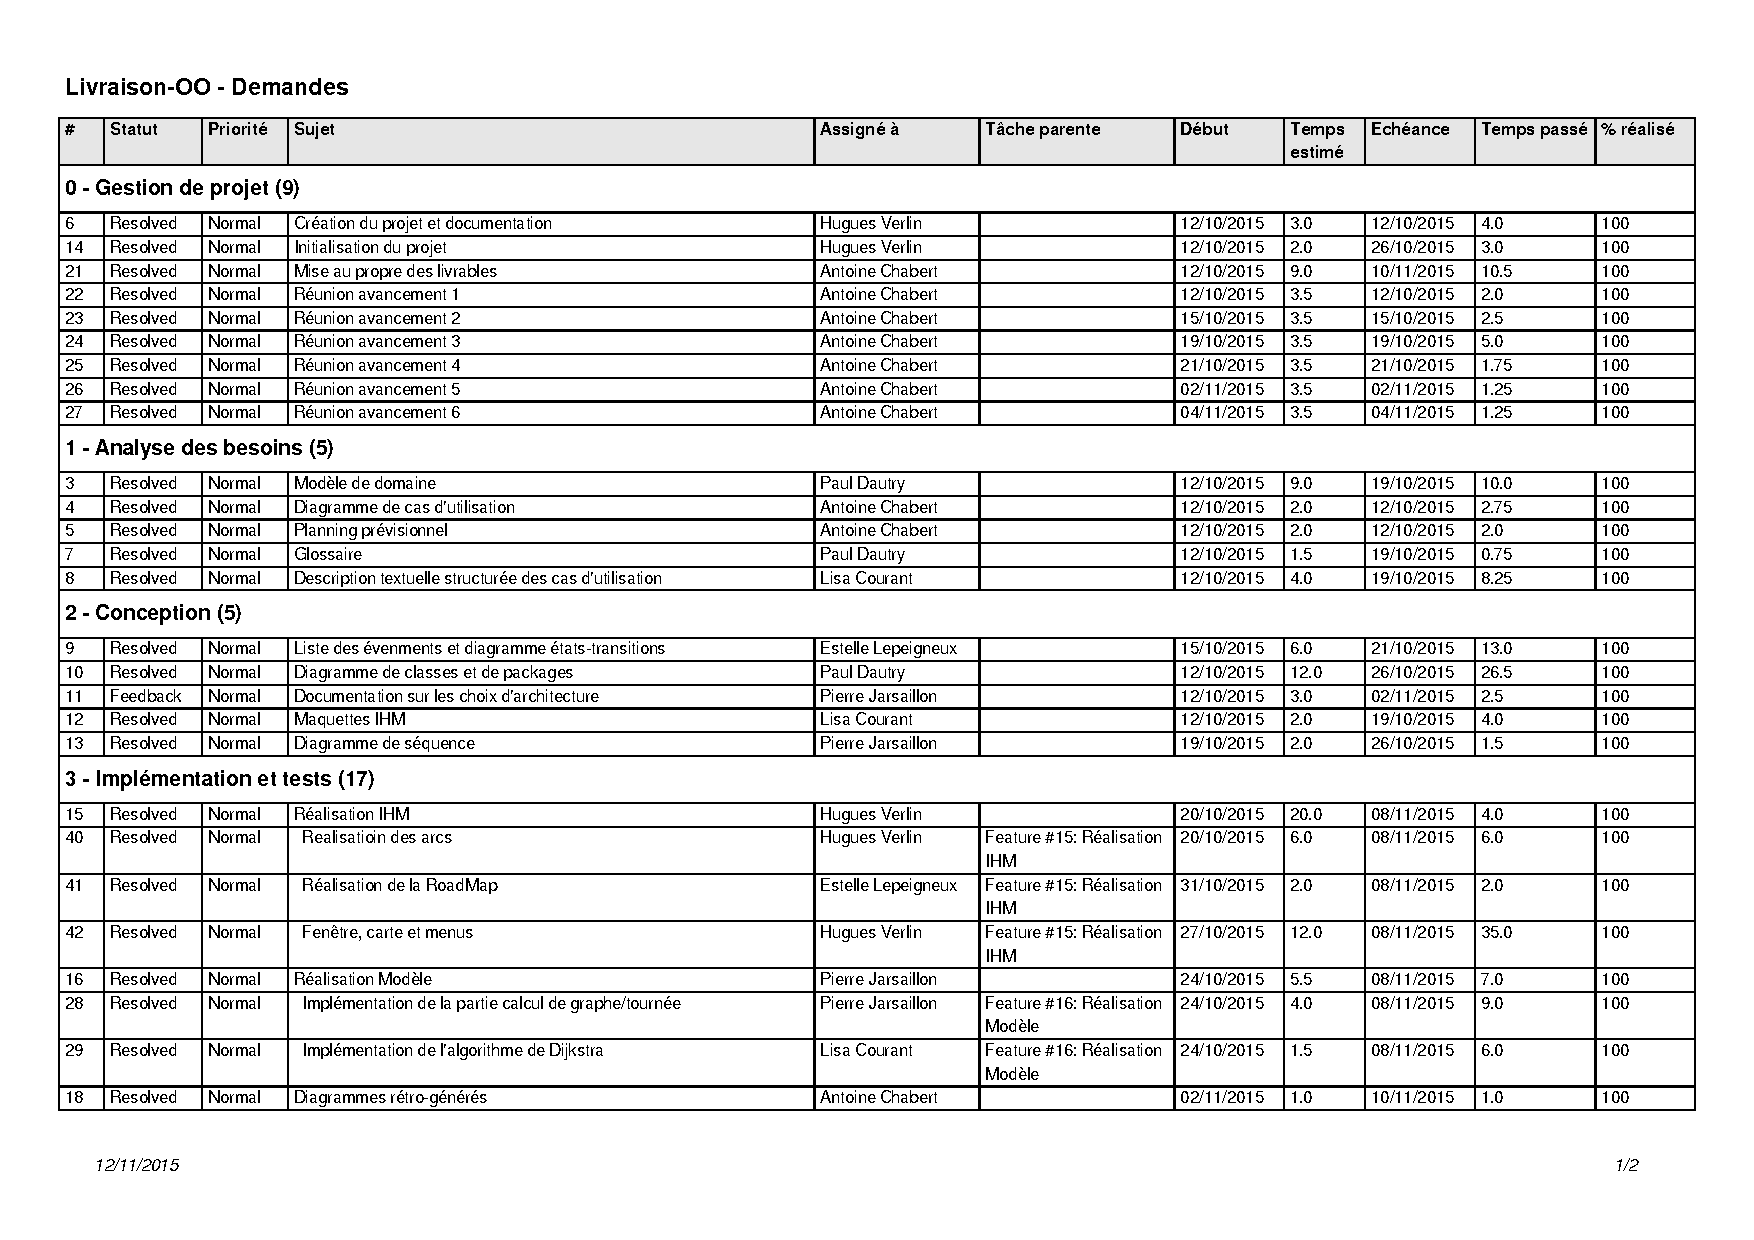
\includepdf[scale=0.8,angle=90,pages={1},pagecommand=\section{Compte-rendu des tâches - Page 1}]{redmine/list-issues-redmine.pdf}
\label{sec:cr-des-taches-redmine}
\includepdf[scale=0.8,angle=90,pages={2},pagecommand=\section{Compte-rendu des tâches - Page 2}]{redmine/list-issues-redmine.pdf}

\section{Détails des temps passés}
\label{sec:details-des-temps-passes}

\begin{figure}[H]
\centering
\noindent\scalebox{0.6}{\pgfplotstabletypeset[
    col sep=semicolon,
    string type,
    columns={Utilisateur,Demande,Temps total},
    columns/Utilisateur/.style={column name=Utilisateur, column type={|l}},
    columns/Demande/.style={column name=Demande, column type={|l}},
    columns/2015/.style={column name=2015, column type={|l}},
    columns/Temps total/.style={column name=Temps Total (heures), column type={|r|}},
    every head row/.style={before row=\hline,after row=\hline},
    every last row/.style={before row=\hline,after row=\hline},
    ]{redmine/users-time-by-issue.csv}}
\caption{Temps passés par personne}
\end{figure}

%%% End document
\end{document}
